\chapter{Many-body Quantum Mechanics} \label{chp:manybody}
\epigraph{We have to remember that what we observe is not nature in itself but
	nature exposed to our method of questioning.}{Werner Heisenberg, \cite{heisenberg_across_1990}}
\begin{figure}[H]
	\centering
	\captionsetup[subfigure]{labelformat=empty}
	\copyrightbox[l]{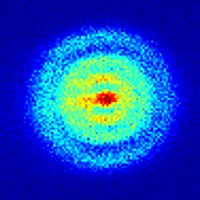
\includegraphics[scale=3]{../Images/art_quantum.jpg}}{Physical review letters,\\ 110, 213001 (2013)}
	\caption{The first photograph of a hydrogen atom was captured by an ultra sensitive camera in 2013. One can actually see the probability distribution $|\Psi(\bs{x})|^2$ with the naked eye. Published by \citet{stodolna_hydrogen_2013} with the title \textit{Hydrogen atoms under magnification}.}
\end{figure}

\sloppy
In the previous chapter, the quantum mechanics of single particles were discussed. We presented the time-independent Schrödinger equation, and from that, we obtained a general expression of the energy of a stationary particle. The energy expression of a stationary \textit{system} is almost identical,
\begin{equation}
E_n=\mel{\Psi_n(\bs{X})}{\hat{\mathcal{H}}}{\Psi_n(\bs{X})},
\label{eq:energy}
\end{equation}
but we here use the many-body wave function $\Psi_n(\bs{X})$ of state $n$ with $\bs{X}=\{\bs{x}_1,\bs{x}_2,\hdots,\bs{x}_N\}=\{(\bs{r}_1, \sigma_1), (\bs{r}_2, \sigma_2),\hdots,(\bs{r}_N, \sigma_N)\}$ denoting the collective coordinates and the spins of all the $N$ particles in the system. The Hamiltonian, $\hat{\mathcal{H}}$, defines the system and is given explicitly in the next section. As noted before, the wave function for large systems needs to store an immense amount of information and is therefore impractical or even impossible to deal with. In this section, we will first look at how the many-body Hamiltonian is set up before we have an extensive discussion of how the many-body wave function is constructed.

\section{The electronic Hamiltonian} \label{sec:electronichamiltonian}
We have already seen what the one-body Hamiltonian looks like, and the many-body Hamiltonian is not very different. We recall that it can be split in a kinetic and a potential term,
\begin{equation}
\hat{H}=\hat{T}+\hat{V}
\end{equation}
where $\hat{T}$ is the kinetic energy and $\hat{V}$ is the potential energy. Nevertheless, as we study electrons, they are charged and will therefore interact with each other. For that reason, we need to add an interaction term to the Hamiltonian, which in general is included in the potential term $V=V_{\text{ext}}+V_{\text{int}}$ with $V_{\text{ext}}$ as the external potential and $V_{\text{int}}$ as the interaction potential. In the same way as the nucleus potential, the interaction potential is given by Coulomb's law, for two electrons given by 
\begin{equation}
V_{\text{int}} =k_e\frac{e^2}{r_{12}}
\end{equation}
where $r_{12}$ is the distance between the electrons. For a general system containing $N$ electrons, the total Hamiltonian can therefore be expressed as 
\begin{empheq}[box={\mybluebox[5pt]}]{equation}
\hat{\mathcal{H}}=-\sum_{i=1}^N\frac{\hbar^2}{2m_e}\nabla_i^2+\sum_{i=1}^{N}V_i + \sum_{i=1}^N\sum_{j>i}^Nk_e\frac{e^2}{r_{ij}}
\label{eq:ElectronicHamiltonian}
\end{empheq}
which is the farthest we can go without specifying the external potential $V_i$. $r_{ij}$ is the relative distance between particle $i$ and $j$, defined by $r_{ij}\equiv|\bs{r}_i-\bs{r}_j|$. From now on, we will use atomic units setting $\hbar=m_e=k_e=e=1$, see appendix \ref{app:units} for details.

By putting this Hamiltonian into equation \eqref{eq:energy}, the integral can be split in three terms,
\begin{equation}
\begin{aligned}
E_n&=\sum_{i=1}^N\bigg[-\frac{1}{2}\mel{\Psi_n(\bs{X})}{\nabla_i^2}{\Psi_n(\bs{X})}
+\mel{\Psi_n(\bs{X})}{V_i}{\Psi_n(\bs{X})}
+\sum_{j>i}^N\mel{\Psi_n(\bs{X})}{\frac{1}{r_{ij}}}{\Psi_n(\bs{X})}\bigg]
\end{aligned}
\end{equation}
where the two former ones are the one-body integrals, or \textit{matrix elements}, which we in many cases easily can solve. However, the last term is very tricky to solve, and in fact there are analytical solutions available for the two-particle case only. In other words, a precise evaluation of this integral can usually only be found using numerical methods, which we will have a closer look at in chapter \ref{chp:methods} in conjunction with quantum Monte Carlo methods.

\section{The many-body wave function} \label{sec:wavefunction}
By the first postulate of quantum mechanics presented in section \ref{sec:postulates}, the wave function contains all the information specifying the state of the system. This means that all observable in classical mechanics can in principle also be estimated from the wave function, which makes finding the wave function our aim. As we have seen, we can define the wave function for a single particle, known as the \textit{single-particle function} (SPF), $\psi(\bs{r},\sigma)$. Can we combine the SPFs of the electrons in a system and obtain the many-body wave function? Possibly, the most straight-forward way of doing this is to simply multiply all the SPFs,
\begin{equation}
\Psi(\bs{X})=\psi(\bs{r}_1,\sigma_1)\psi(\bs{r}_2,\sigma_2)\hdots\psi(\bs{r}_N,\sigma_N),
\end{equation}
known as the \textit{Hartree product}. However, this product is generally not correct, as it does not include the required symmetry properties of the many-body wave function. Instead, we can take the symmetry into account by expressing the many-body wave function as a determinant or a permanent, as we will see in section \ref{sec:slater}. In addition to the symmetry properties, there is an array of requirements the wave function needs to meet in order to be physically correct. Some of them are:

\iffalse
We will in this section discuss the symmetry properties of the wave function for bosonic and fermionic systems, and see how the wave function can be set up as a Slater determinant in order to meet these properties. Also, Jastrow factors will be touched, as they are used in quantum Monte Carlo methods to handle the correlations. With that in mind, we approximate the \textit{trial} wave function by a Slater-Jastrow function,
\begin{equation}
\Psi_T(\bs{r};\bs{\theta})=|\hat{D}(\bs{r};\bs{\theta})|J(\bs{r};\bs{\theta}),
\end{equation}
which is an educated guess of the form of the wave function. 
Here the first part, $|\hat{D}(\bs{r};\bs{\theta})|$, is the Slater determinant and $J(\bs{r};\bs{\theta})$ is a Jastrow factor with $\theta$ as some variational parameters. Other quantum many-body methods, such as full configuration interaction and coupled cluster use a linear expansion of Slater determinants to approximate the wave function, while the Hartree-Fock method relies on one single Slater determinant (without any Jastrow factor). Nevertheless, as we will focus on quantum Monte Carlo methods, this chapter will be tailored to the method. 

The trial wave function needs to satisfy some requirements in order to be used in the variational principle, and we thus need to make an educated guess on the wave function where the requirements are fulfilled. The requirements are the following:
\fi

\begin{enumerate}
	\item \textbf{Normalizability:} The wave function needs to be normalizable in order to make physical sense. The total probability should always be 1, and a wave function that cannot be normalized will not have a finite total probability. The consequence is that the wave function goes to zero when the positions get large, $\Psi(x\rightarrow\pm\infty)\rightarrow 0$. 
	
	\item \textbf{Cusp condition:} The cusp condition, or the Kato theorem, states that the wave function should have a cusp where the potential explodes. An example on this is when electrons come close to each other, i.e., the electron-electron cusp.
	
	\item \textbf{Symmetry and anti-symmetry:} The wave function needs to be either symmetric or anti-symmetric under the exchange of two coordinates, dependent on whether the electrons are fermions or bosons. This is the statement of the sixth postulate, which will be further explained in the next section.
\end{enumerate}

\subsection{Anti-symmetry and the Pauli principle} \label{sec:symmetry}
Symmetry and anti-symmetry are central concepts in quantum mechanics, and often one can use symmetry arguments to simplify expressions and calculations. In this section, we will look at the symmetry and anti-symmetry properties of the wave function and discuss how it can be used to define a wave function in the next section.

Assume that we have a permutation operator, $\hat{P}(i\rightarrow j)$, which exchanges the coordinates of the particles $i$ and $j$ in the many-body wave function containing $M$ particles,
\begin{equation}
\hat{P}(i\rightarrow j)\Psi_n(\bs{x}_1,\hdots,\bs{x}_i,\hdots,\bs{x}_j,\hdots,\bs{x}_M)=p\Psi_n(\bs{x}_1,\hdots,\bs{x}_j,\hdots,\bs{x}_i,\hdots,\bs{x}_M),
\end{equation}
where $p$ is just a factor which comes from the transformation. If we again apply the $\hat{P}$ operator, we should switch the same coordinates back, and we expect to end up with the initial wave function. For that reason, $p$ must be either +1 or -1. \footnote{Actually, in two-dimensional systems a third possibility is allowed which gives an \textit{anyon}. The theory on this was developed by \citet{leinaas_one_1977} during the 1970s.} The particles that have an anti-symmetric wave function under the exchange of two coordinates are called fermions, named after Enrico Fermi, and as discussed before, they have half-integer spin. On the other hand, the particles that have a symmetric wave function under the exchange of two coordinates are called bosons, named after Satyendra Nath Bose, and have integer spin. A consequence of the anti-symmetric wave function is that two identical fermions cannot occupy the same state at the same time, known as the Pauli principle. This means that identical fermions even in the ground state (at zero temperature) spread over multiple states, and in the next section, we will see how this principle is baked into the wave function through a Slater determinant. 

\subsection{The Slater determinant} \label{sec:slater}
For a system of many particles, we can define a many-body wave function, which is a composition of all the SPFs and contains all the information about the system as the first postulate requires. For fermions, we need to combine the SPFs such that the Pauli principle is fulfilled at all times, which can be accomplished by a determinant. 

Consider a system of two identical fermions with SPFs $\psi_1(\bs{r},\sigma)$ and $\psi_2(\bs{r},\sigma)$ with coordinates and spin $\boldsymbol{r}_1,\sigma_1$ and $\boldsymbol{r}_2,\sigma_2$ respectively. The way we define the wave function of the system is then
\begin{equation}
\begin{aligned}
\Psi(\bs{X})&=\frac{1}{\sqrt{2}}
\begin{vmatrix}
\psi_1(\boldsymbol{r}_1,\sigma_1) & \psi_2(\boldsymbol{r}_1,\sigma_1)\\
\psi_1(\boldsymbol{r}_2,\sigma_2) & \psi_2(\boldsymbol{r}_2,\sigma_2)
\end{vmatrix}\\
&=\frac{1}{\sqrt{2}}\Big[\psi_1(\boldsymbol{r}_1,\sigma_1)\psi_2(\boldsymbol{r}_2,\sigma_2)-\psi_2(\boldsymbol{r}_1,\sigma_1)\psi_1(\boldsymbol{r}_2,\sigma_2)\Big],
\end{aligned}
\end{equation}
which is automatically set to zero if the particles happen to be at the same position and have the same spin at the same time. If the particles, on the other hand, have different spins, they are allowed to appear at the same position at the same time and the determinant will not cancel. For larger systems, the Slater determinant is constructed in the same way as above, and any pair of identical particles located in the same state will make the determinant collapse. A Slater determinant containing $N$ electrons reads
\begin{equation}
\Psi(\bs{X})=\frac{1}{\sqrt{N!}}
\begin{vmatrix}
\psi_1(\boldsymbol{r}_1,\sigma_1) & \psi_2(\boldsymbol{r}_1,\sigma_1) & \hdots & \psi_N(\boldsymbol{r}_1,\sigma_1)\\
\psi_1(\boldsymbol{r}_2,\sigma_2) & \psi_2(\boldsymbol{r}_2,\sigma_2) & \hdots & \psi_N(\boldsymbol{r}_2,\sigma_2)\\
\vdots & \vdots & \ddots & \vdots \\
\psi_1(\boldsymbol{r}_N,\sigma_N) & \psi_2(\boldsymbol{r}_N,\sigma_N) & \hdots & \psi_N(\boldsymbol{r}_N,\sigma_N)
\end{vmatrix}
\end{equation}
where the $\psi(\bs{r},\sigma)$ is the tensor product between the radial part $\phi(\bs{r})$ and the spin part $\xi(\sigma)$,
\begin{equation}
\psi(\bs{r},\sigma)=\phi(\bs{r})\otimes\xi(\sigma).
\end{equation}
In section \ref{sec:slaterdeterminant}, it is shown that the Slater determinant can be split in a spin-up part and a spin-down part such that the spin-dependency $\xi(\sigma)$ can be omitted. For that reason, we can define a basis set consisting of the spatial parts only, discussed in the next section. 

As a note, we will in the rest of this thesis use $\Psi$ as the many-particle wave function, $\psi$ are the SPFs, and $\phi$ is the spatial part of the SPF. $\xi$ will be reserved the spin part of the SPFs, but will often be omitted as the spin-part can be factorized out. Sometimes it is appropriate to split up the many-particle wave function, and we will, in that case, denote each part by $\Psi_i$ where $i$ is an index associated with the particular element. Lastly, the basis functions will be denoted by $\varphi$, which we will discuss in the next section.

\subsection{Basis set} \label{sec:basisset}
In quantum chemistry, a basis set is a set of basis functions, which often are called the atomic orbitals.  Generally, a basis function should not be confused with a single-particle function, as a single-particle function is a linear combination of basis functions, and are thus often called the molecular orbitals. Commonly used atomic orbitals are Pople basis sets (in the form of x-yz G), correlation-consistent basis sets (in the form of cc-pVNZ) and Slater-type orbitals (in the form of STO-nG), where all are built on Gaussian functions. Gaussian functions are preferred as they allow efficient implementations of post Hartree-Fock methods.

In our work, however, the single-particle functions are often the basis functions, as we in most of the cases do not expand our single-particle functions $\psi(\bs{r},\sigma)$ in a basis. Our single-particle functions are typically the solution of the non-interacting system, and as the Jastrow factor is supposed to deal with the interaction, we use the same functions for the interacting case as well.

A common notation is to use the Greek letter $\varphi$ for the atomic orbitals and $\psi$ for the molecular orbitals, such that single-particle functions can be obtained from an expansion of the $N$ basis functions $\{\varphi_1(\bs{r}),\varphi_2(\bs{r}),\hdots\varphi_N(\bs{r})\}$ in the manner of
\begin{equation}
\phi_i(\bs{r})=\sum_{j=1}^Nc_{ji}\varphi_j(\bs{r}),
\label{eq:expansion}
\end{equation}
where $c_{ij}$ are the coefficients to be found. There are different approaches to obtain these coefficients, where the popular Hartree-Fock algorithm generates $c_{ij}$'s in order to find the optimal Slater determinant. The larger basis, the more accurate results we will get but at a gradually higher cost. The actual functions used in this work are presented in the next chapter, \ref{chp:systems}, and linked to their respective systems. 

\subsection{Modeling the cusp} \label{sec:cusp}
From electrostatics, we know that identical, charged particles will repulse each other. This means that the probability of finding two particles close to each other should be low, which needs to be baked into the wave function. To estimate the observable accurately, it is crucial to model the electron-electron cusp correctly.

Different methods attack this challenge in different ways. The Hartree-Fock method attempts to construct an optimal single Slater determinant by expanding the molecular orbitals in atomic orbitals, like shown in equation \eqref{eq:expansion}. The coefficients are determined such that the energy is minimized, which is performed by the Hartree-Fock algorithm \cite{hartree_wave_1928, fock_selfconsistent_1930}. Then, we only need to deal with a Slater determinant, and as the correlations are not given explicitly, the Hartree-Fock theory is often called a mean-field theory. Further, we have a bunch of post Hartree-Fock methods, like configuration interaction and the coupled cluster method, which utilize the Hartree-Fock basis, but express the wave function as a linear combination of Slater determinants, where the correlations are determined by the coefficients \cite{daniel_crawford_introduction_2007}. If a sufficient number of Slater determinants are included in the linear combination, both the methods are capable of providing exact results. However, since the scaling goes as $N!$ and $N^6$ respectively, this is possible only for very small systems.

The variational Monte Carlo (VMC) method, which we have implemented in this work, models the electron-electron cusp in a totally different way. We there define a \textit{trial wave function}, which consists of one or more Slater determinants and a Jastrow factor, where the latter is assumed to account for the correlations. In that way, the Slater determinants are used only to account for the Pauli principle only. The Jastrow factor will be discuss further in section \ref{sec:jastrow}.

However, our primary focus in this work is to see if we can use machine learning to reduce the need of physical intuition. Our hope is that the method will be able to model the cusp correctly without prior knowledge about the correlations. In the first place, we will try to construct a flexible Slater determinant based on neural network, which also models the correlations.

\section{Electron density} \label{sec:electrondensity}
In quantum many-body computations, the electron density is frequently calculated, and there are several reasons for that. First, the electron density can be found experimentally, such that the calculations can be benchmarked. Second, the electron density is very informative, since information about all particles can be gathered in one plot. The $P$-body electron density is defined by the multi-dimensional integral over the probability density function of all the particles but $P$, for a normalized wave function represented by
\begin{empheq}[box={\mybluebox[5pt]}]{equation}
\label{eq:electron_density}
\rho_P(\bs{r}_1,\hdots,\bs{r}_P)=N\int_{-\infty}^{\infty}d\bs{r}_{P+1}\hdots d\bs{r}_N |\Psi(\bs{r}_1,\hdots \bs{r}_N)|^2
\end{empheq}
where $P\leq N$. This integral is in general really tricky so solve, and it can be found analytically for just a few realistic systems. For other systems, we need to solve the integral numerically, and we will in chapter \ref{chp:methods} describe how this can be done using Monte Carlo integration. The density should not be normalized to unit both when it is calculated analytically and numerically, but to the number of particles, i.e.,
\begin{equation}
\int_{-\infty}^{\infty}d\bs{r}_{1}\hdots d\bs{r}_P\Big[\rho_P(\bs{r}_1,\hdots,\bs{r}_P)\Big]=N.
\end{equation}

As we cannot pinpoint a particle in quantum mechanics, i.e., it is impossible to distinguish two identical particles in any way, the electron density is the same no matter which particles we decide to leave out. In equations, we always leave out the first $P$ particles, but we could also, for instance, have left out the $P$ last particles and so forth.

So, what does the electron density tell us? The one-body density, $\rho_1(\bs{r}_1)$, is the most applied electron density and is sometimes simply referred to as the electron density. It gives the probability density of finding an electron throughout the space, and give insight about how the particles are distributed in the system. On the other hand, the two-body density. $\rho_2(\bs{r}_1,\bs{r}_2)$, becomes a two-dimensional function and is therefore often expressed as a matrix. It gives the probability density of finding an electron throughout the space, given the coordinates of another particle. It, therefore, contains information about how the particles distribute relative to each other and is essential when we want to study the pairwise interaction. In systems with strong forces, such as nuclear systems, the three-body interactions become important and then it also makes sense to look at the three-body density $\rho_3(\bs{r}_1, \bs{r}_2, \bs{r}_3)$. For closed-shell circular quantum dots the radial electron density profile is often preferred as the density then also is circular and independent of the angle. 

For non-interacting systems, the wave function is trivially separable with respect to the different particles. In those cases one can easily find the electron density analytically, since the functions of coordinates which we do not integrate over can be factorized out of the integral,
\begin{equation}
\begin{aligned}
\rho_P(\bs{r}_1,\hdots,\bs{r}_P)&=\int_{-\infty}^{\infty}d\bs{r}_{P+1}\hdots d\bs{r}_N |\Psi(\bs{r}_1),\hdots \Psi(\bs{r}_N)|^2\\
&=\int_{-\infty}^{\infty}d\bs{r}_{P+1}\hdots d\bs{r}_N |\Psi(\bs{r}_1)|^2\hdots |\Psi(\bs{r}_N)|^2\\
&=|\Psi(\bs{r}_1)|^2\hdots |\Psi(\bs{r}_P)|^2\underbrace{\int_{-\infty}^{\infty}d\bs{r}_{P+1}|\Psi(\bs{r}_{P+1})|^2\hdots\int_{-\infty}^{\infty}d\bs{r}_{N}|\Psi(\bs{r}_{N})|^2}_{=1}\\
&=|\Psi(\bs{r}_1)|^2\hdots |\Psi(\bs{r}_P)|^2,
\end{aligned}
\end{equation}
where we have assumed that the wave functions are normalized. This result has no scientific importance, but will be used to validate the implementation of the electron density in the code, see section \ref{sec:norepulsive}.

\subsection{Wigner crystals} \label{sec:wigner}
A Wigner crystal is a solid phase where electrons maximize the distance to each other in order to minimize the potential energy. As Coulomb's law gives the interaction potential, the potential is minimized when the distances between the electrons are maximized. In one-dimensional systems, the electrons are thus found at discrete locations, such that they form an evenly spaced lattice. In two-dimensional systems, the Wigner crystals form triangular lattices which are known to be the configuration that maximizes the distance in a limited space, and in three-dimensional systems, the electrons form so-called body-centered cubics. The phenomenon occurs only when the potential energy dominates the kinetic energy since the electrons then are almost "at rest" and external forces are not strong enough to push the electrons close to each other. 

If the concept still is unclear, imagine Norwegians waiting for the metro. In the nature of the people, the Norwegians always want to maximize the distance to each other, meaning that they form triangular lattices on the metro station. In extreme cases, this is equivalent to the Wigner crystals.


